In order to replicate more accurately the expected behavior from cells and microparticles, Polystyrene microbeads are added to the 15\% saline solution. This SUT at 22 $^{\circ}$C is then passed in a 180 $\mu m$ wide microchannel and the impedance is measured for the single square excitation frequency of 1 MHz just as before. The sampling rate is set to a variable burst rate of 5.461 kSps and low-frequency constant rate of 30Hz to not overload the CPU (see \autoref{sec:MCU}). This means that the impedance is measured at fixed low-frequency of 30Hz until a significant difference is observed in the real components of any of the two electrode pairs. When such a difference is observed, a burst of 16 measurement points will be sampled at once at a frequency of 5.461 kSps. This method produces regularly fixed datapoint and dense bursts of data when a particle is detected. The raw signals obtained in this way are shown in \autoref{fig:BeadsADCResponse}. \par
\begin{figure}[h]
\centering
\begin{subfigure}{0.49\textwidth}
\centering
    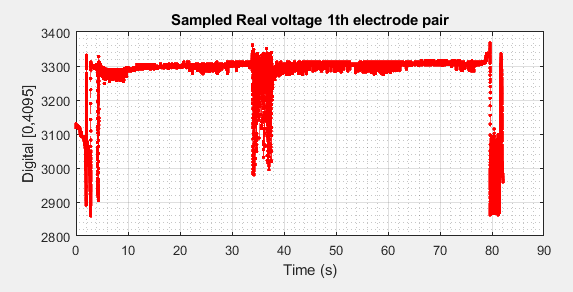
\includegraphics[width=0.99\linewidth]{BeadsReal1}
    \caption{Real response of the first electrode pair.}
    \label{fig:BeadsReal1}
\end{subfigure}
\begin{subfigure}{0.49\textwidth}
\centering
    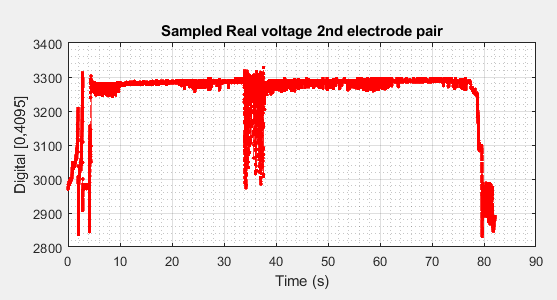
\includegraphics[width=0.99\linewidth]{BeadsReal2}
    \caption{Real response of the second electrode pair.}
    \label{fig:BeadsReal2}
\end{subfigure}
\vskip\baselineskip
\centering
\begin{subfigure}{0.49\textwidth}
\centering
    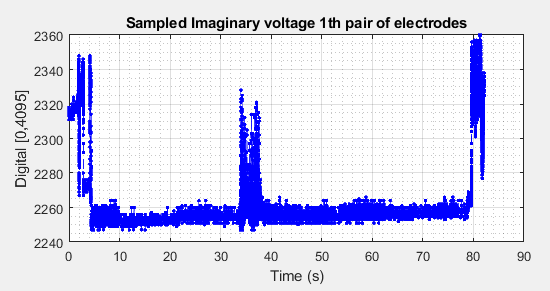
\includegraphics[width=0.99\linewidth]{BeadsImaginary1}
    \caption{Imaginary response of the first electrode pair.}
    \label{fig:BeadsImaginary1}
\end{subfigure}
\begin{subfigure}{0.49\textwidth}
\centering
    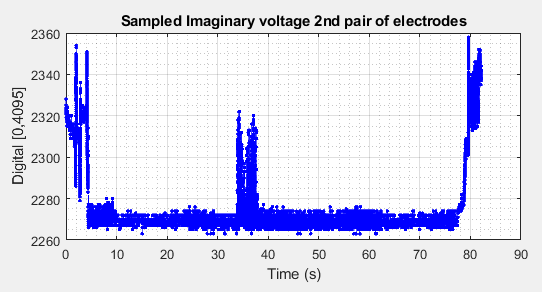
\includegraphics[width=0.99\linewidth]{BeadsImaginary2}
    \caption{Imaginary response of the second electrode pair.}
    \label{fig:BeadsImaginary2}
\end{subfigure}
\caption{Raw signals obtained at the ADCs of the impedance sensing system for saline water at 22 $^{\circ}$C mixed with Polystyrene microbeads of sizes between 10 and 90 $\mu m$  excited by a square excitation signal of frequency 1MHz in a 180 $\mu m$ wide microchannel.}
\label{fig:BeadsADCResponse}
\end{figure}

Let's numerically process the impedance magnitude and phase so that they become easier to analyze. Firstly, the mean values of the magnitude and phase of the two electrode pairs are taken out using wavelet decomposition. The signal is then de-noised, low-pass filtered, and smoothed so that the impedance spikes due to the particles are easier to recognize. The difference between the two electrode pairs are finally calculated since the object of interest in IFC is the amplitude difference and widths of the half-sine created by the impedance difference of the particle passing between two electrode pairs. The full signals are shown in \autoref{fig:BeadsImpedanceDifference}. \par
\begin{figure}[h]
\centering
\begin{subfigure}{0.99\textwidth}
\centering
    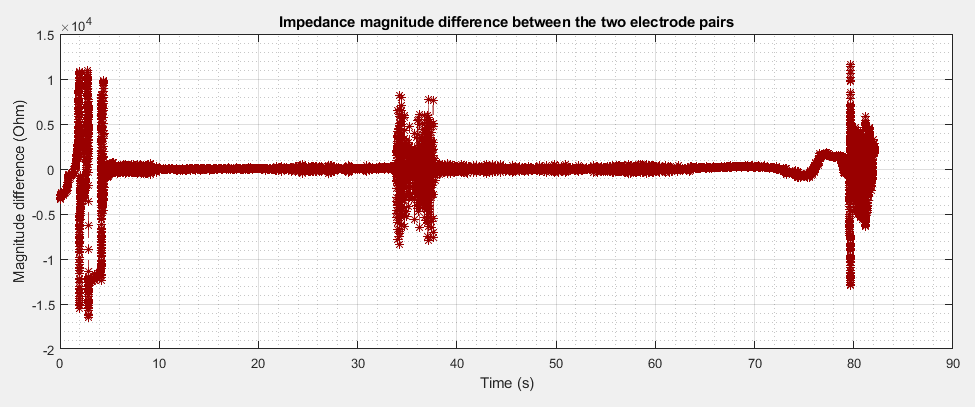
\includegraphics[width=0.99\linewidth]{BeadsMagnitudeDifference}
    \caption{Magnitude difference of the two electrode pairs.}
    \label{fig:BeadsMagnitudeDifference}
\end{subfigure}
\begin{subfigure}{0.99\textwidth}
\centering
    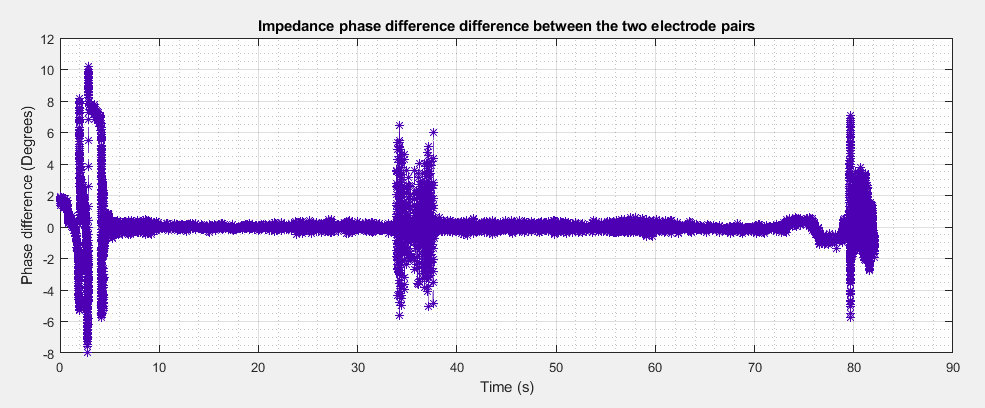
\includegraphics[width=0.99\linewidth]{BeadsPhaseDifference}
    \caption{Phase difference of the two electrode pairs.}
    \label{fig:BeadsPhaseDifference}
\end{subfigure}
\caption{Filtered impedance difference between the two electrode pairs measured as a function of time for saline water at 22 $^{\circ}$C mixed with Polystyrene microbeads of sizes between 10 and 90 $\mu m$  excited by a square excitation signal of frequency 1MHz in a 180 $\mu m$ wide microchannel. Different behaviors are observed at different timestamps of the signal.}
\label{fig:BeadsImpedanceDifference}
\end{figure}

Now, what exactly is happening with the electrode and solution to produce such curves? In the 82 seconds of the measurements, a couple of things happenned in the channel:
\begin{enumerate}
  \item The electrodes are initially relatively dry, meaning that the channel may have a residual liquid in it but the electrodes are not in full contact with it. This case-situation is associated to high values of impedance compared to the the impedance of the solution and is associated with a high variability of the measured impedance since the impedance measured on the electrodes is quickly modified by the shape and position of the residual liquid droplets that are found on the electrodes. This first situation is shown in \autoref{fig:BeadsImpedanceDifference5s}.
  \item The SUT then flows in the channel at a high speed. At this stage, between 5s and 10s, microparticles are flowing at such a high flow-rate in the channel that only 2 or 3 points are recorded when a particle passes in the channel. In other words, the sampling frequency is not high enough to accomodate such high flow velocity that only two or three samples are taken between the moment the particle arrives at the electrode pair and the moment it passed it. This behavior is shown in \autoref{fig:BeadsMagnitudeDifferenceZoomed10s}. Beads passed in the channel and the full-sine patterns are observed for six of them. 
  \item From the 10th to the 20th second, the liquid flow was stopped so that no beads would pass the electrodes. It is possible to see in \autoref{fig:BeadsImpedanceDifference20s} that no full-sine waves are observed in the impedance magnitude signal. 
  \item From the 22th to the 32th second, the liquid flow is resumed, at a more reasonable flow velocity this time. Full-sine waves with adequate numbers of samples are obtained, as shown in \autoref{fig:BeadsImpedanceDifference30s}. The beads generally produce impedance differences of less than 800 $\Omega$.
  \item From the 33th to the 38th second, air bubbles are introduced in the channel. These bubbles create massive impedance differences which are fairly easy to differentiate from the beads, as shown in \autoref{fig:BeadsImpedanceDifference38s}. The detection algorithm will discriminate between them later on. 
  \item From the 40th to the 63th seconds, particles flow in the channel at decent variable flow-rate. Some great particle recognition are observes, such as the ones in \autoref{fig:BeadsGreatDetection}. 
  \item After that, the liquid is flow is stopped for a moment, and the liquid is then flown out of the channel. A behavior similar to the beginning is observed, when the electrodes were only partially in contact with the SUT. 
\end{enumerate}

\begin{figure}[h]
\centering
\begin{subfigure}{0.99\textwidth}
\centering
    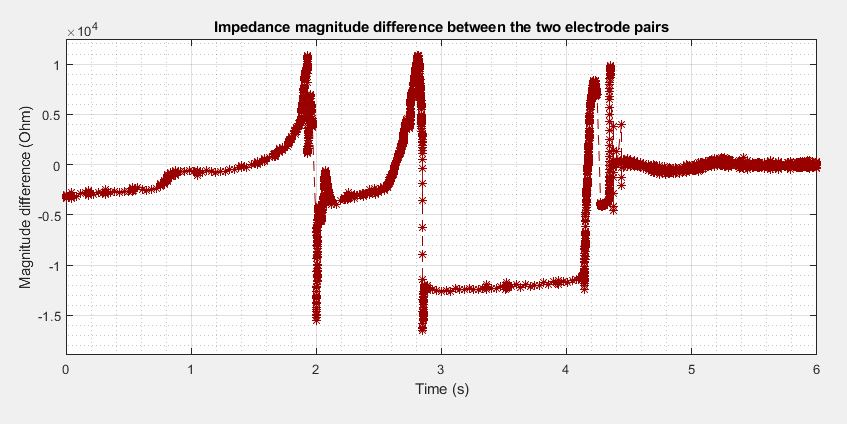
\includegraphics[width=0.9\linewidth]{BeadsMagnitudeDifference5s}
    \caption{Magnitude difference of the two electrode pairs.}
    \label{fig:BeadsMagnitudeDifference5s}
\end{subfigure}
\begin{subfigure}{0.99\textwidth}
\centering
    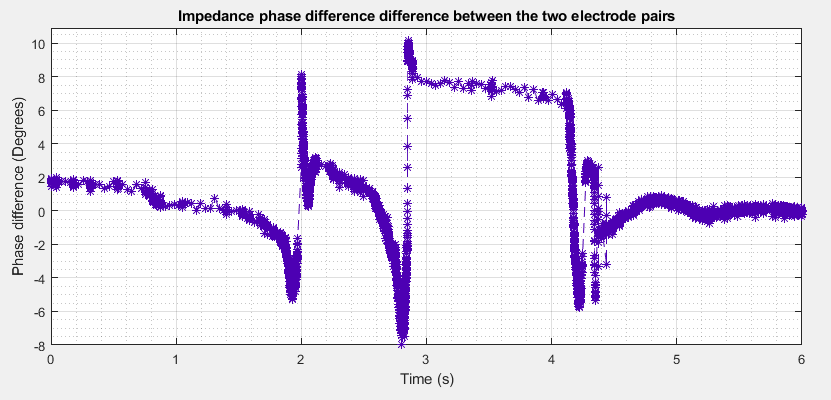
\includegraphics[width=0.9\linewidth]{BeadsPhaseDifference5s}
    \caption{Phase difference of the two electrode pairs.}
    \label{fig:BeadsPhaseDifference5s}
\end{subfigure}
\caption{[0s to 6s] A region of partially wet electrodes and air bubbles observed from the filtered impedance difference between the two electrode pairs obtained from the SUT.}
\label{fig:BeadsImpedanceDifference5s}
\end{figure}

\begin{figure}[h]
\centering
\begin{subfigure}{0.99\textwidth}
\centering
    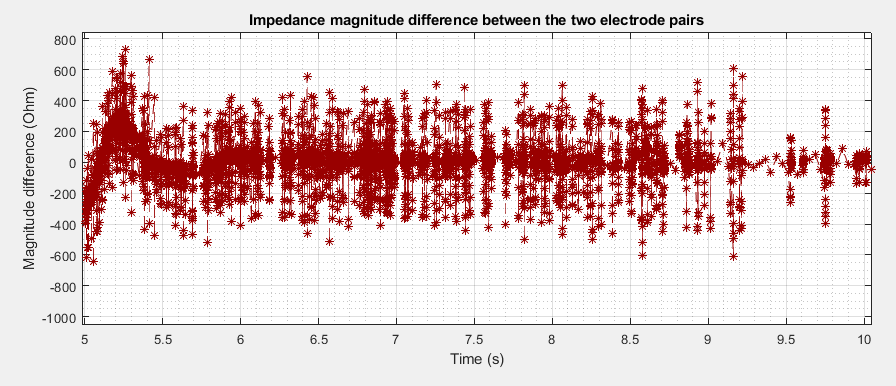
\includegraphics[width=0.99\linewidth]{BeadsMagnitudeDifference10s}
    \caption{Full signal.}
    \label{fig:BeadsMagnitudeDifference10s}
\end{subfigure}
\begin{subfigure}{0.99\textwidth}
\centering
    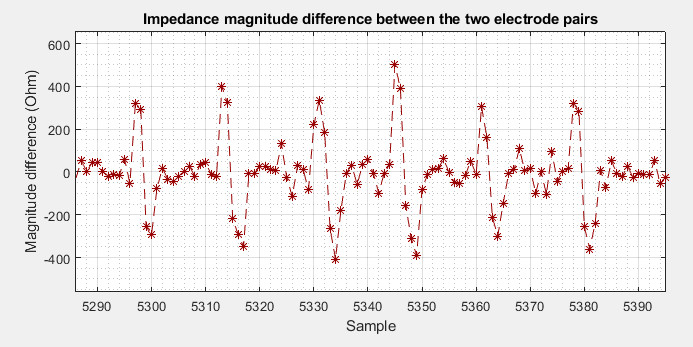
\includegraphics[width=0.99\linewidth]{BeadsMagnitudeDifferenceZoomed10s}
    \caption{Signal zoomed on the patterns created by 6 beads.}
    \label{fig:BeadsMagnitudeDifferenceZoomed10s}
\end{subfigure}
\caption{[5s to 10s] A region of high flow velocity with beads observed from the filtered impedance magnitude difference between the two electrode pairs obtained from the SUT. Not many samples are taken for each particle since they flow too quickly.}
\label{fig:BeadsImpedanceDifference10s}
\end{figure}

\begin{figure}[h]
\centering
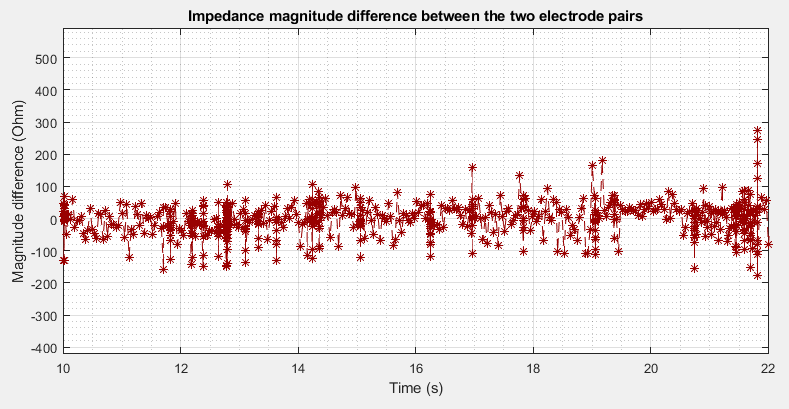
\includegraphics[width=0.99\linewidth]{BeadsMagnitudeDifference20s}
\caption{[10s to 20s] A region of no flow nor bubbles observed from the filtered impedance magnitude difference between the two electrode pairs obtained from the SUT. The spikes represent the baseline level of noise.}
\label{fig:BeadsImpedanceDifference20s}
\end{figure}

\begin{figure}[h]
\centering
\begin{subfigure}{0.99\textwidth}
\centering
    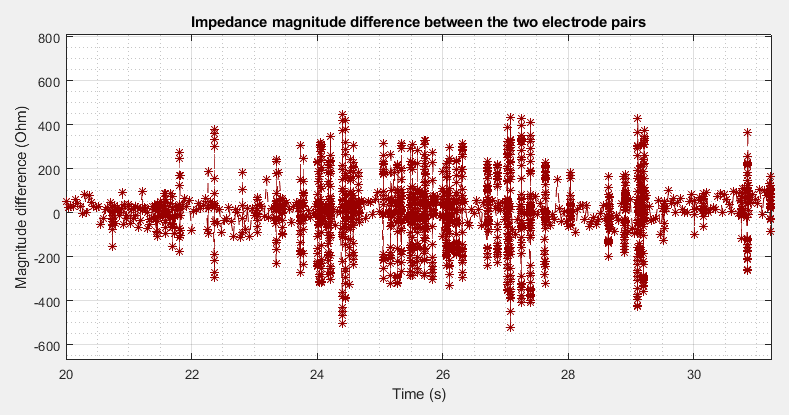
\includegraphics[width=0.99\linewidth]{BeadsMagnitudeDifference30s}
    \caption{Full signal.}
    \label{fig:BeadsMagnitudeDifference30s}
\end{subfigure}
\begin{subfigure}{0.99\textwidth}
\centering
    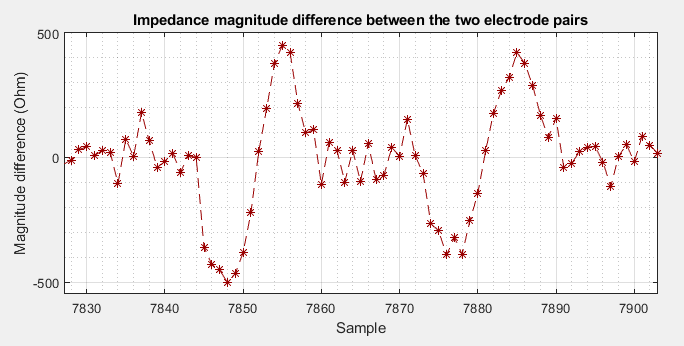
\includegraphics[width=0.99\linewidth]{BeadsMagnitudeDifferenceZoomed30s}
    \caption{Signal zoomed on the patterns created by 6 beads.}
    \label{fig:BeadsMagnitudeDifferenceZoomed30s}
\end{subfigure}
\caption{[20s to 33s] Beads pattern observed from the filtered impedance magnitude difference between the two electrode pairs obtained from the SUT. This time the beads flow slowly and more datapoints are taken for one bead.}
\label{fig:BeadsImpedanceDifference30s}
\end{figure}

\begin{figure}[h]
\centering
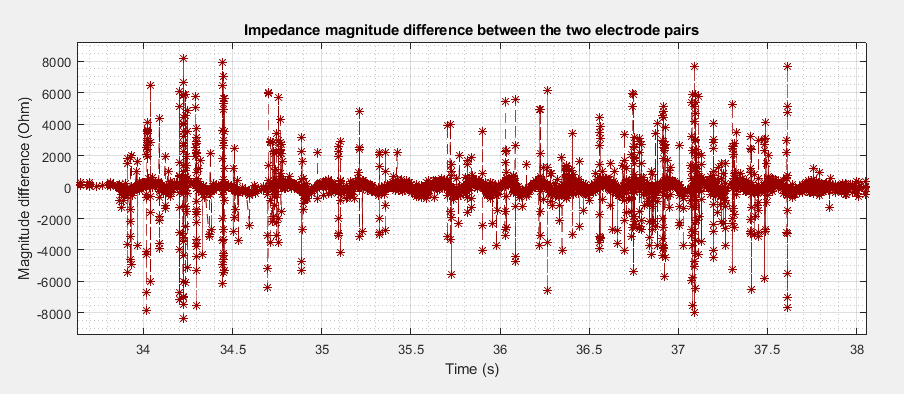
\includegraphics[width=0.99\linewidth]{BeadsMagnitudeDifference38s}
\caption{[33s to 38s] Bubbles observed from the filtered impedance magnitude difference between the two electrode pairs obtained from the SUT. The magnitude difference created by bubbles is really high, making them easy to discriminate from the beads.}
\label{fig:BeadsImpedanceDifference38s}
\end{figure}

\begin{figure}[h]
\centering
\begin{subfigure}{0.49\textwidth}
\centering
    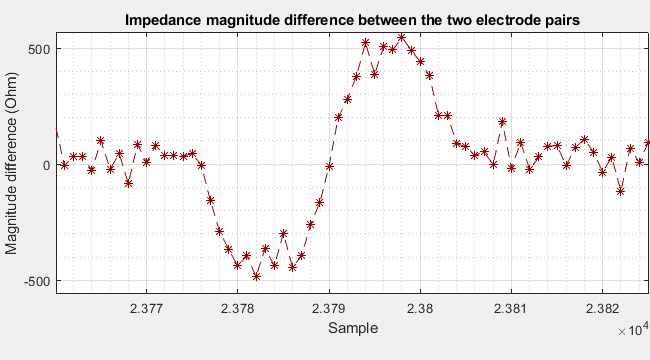
\includegraphics[width=0.99\linewidth]{BeadsGreatDetection1}
    \caption{Great pattern obtained from 1 beads.}
    \label{fig:BeadsGreatDetection1}
\end{subfigure}
\begin{subfigure}{0.49\textwidth}
\centering
    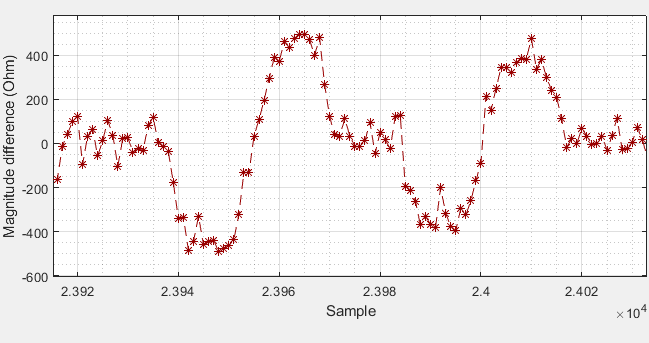
\includegraphics[width=0.99\linewidth]{BeadsGreatDetection2}
    \caption{Great patterns obtained from 2 beads.}
    \label{fig:BeadsGreatDetection2}
\end{subfigure}
\caption{Examples of great microbeads patterns obtained from the SUT.}
\label{fig:BeadsGreatDetection}
\end{figure}

A particle detection algorithm is used on this dataset to recover the positions of the peaks. A peak detection algorithm is first used, followed by a Weak Supervision approach  \cite{ratner2017snorkel} using Snorkel to discriminate between the peaks obtained from bubbles, from the peaks obtained from beads, from the outliers and irregular data. \autoref{fig:BeadsPeakDetection} show the dataset with the detected peaks for a couple of beads. \par
\begin{figure}[h]
\centering
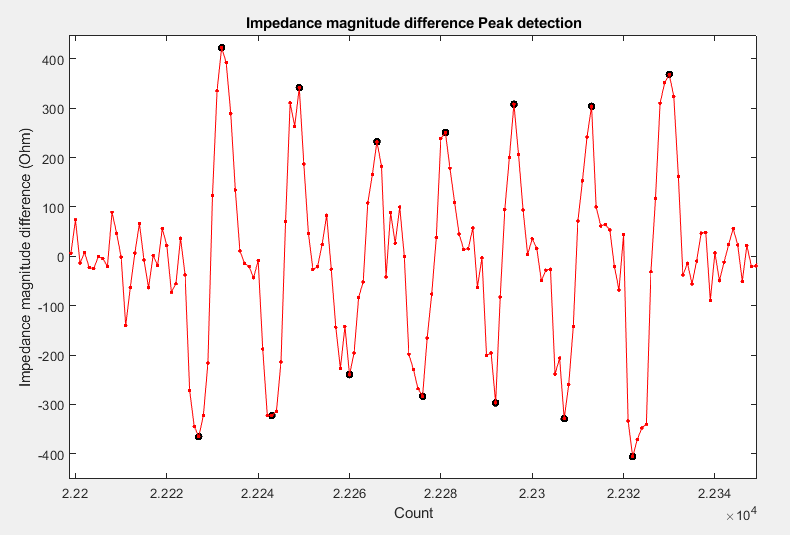
\includegraphics[width=0.8\linewidth]{BeadsPeakDetection}
\caption{Detected peaks from the filtered impedance magnitude difference between the two electrode pairs obtained from the SUT.}
\label{fig:BeadsPeakDetection}
\end{figure}

With these peak locations, it is possible to recover the amplitude and widths of the patterns, which are used to estimate the microbeads velocity and sizes, as explained in \autoref{sec:IFC} with \autoref{eq:sizeEstimation} and \autoref{eq:VelocityEstimation}. As an example, the pattern of \autoref{fig:BeadsGreatDetection1} will be studied. It has a positive impedance magnitude difference of 510 $\Omega$ and a negative impedance magnitude of 490 $\Omega$. Its $G$ constant is not known at this moment, but will be estimated using Big Data in \autoref{sec:BigData} as $G=7$. This leads us to a diameter value of 70 $\mu$m, which is adequate considering that this peak was fairly important and that the beads are of sizes between 10 $\mu$m and 90 $\mu$m. To calculate the beads velocity, the time it took for the particle to pass the electrodes is measured. This time is found to be 2.2 $\mu$s. The distance the bead had to flow through in that time, which is the distance separating the electrode pairs is divided to that time to obtain the particle velocity. That distance is of 406 $\mu$m. This leads to a velocity of 0.185 m/s.